%\title{Overleaf Memo Template}
% Using the texMemo package by Rob Oakes
\documentclass[letter,12pt]{texMemo}
\usepackage[english]{babel}
\usepackage{graphicx, outlines, float}
\pagenumbering{gobble}

%% Edit the header section here. To include your
%% own logo, upload a file via the files menu.
\memoto{Whom It May Concern}
\memofrom{Kyle Salitrik}
\memosubject{Preliminary Scheduling Database Design}
\memodate{\today}
%\logo{
\includegraphics[width=0.3\textwidth]{Overleaf-logo.jpg}}
\graphicspath{{./figures/}}

\begin{document}
\maketitle
Included in this document are figures of the tables that will be represented within the database system. Each table will be explained individually in full and it will be noted which tables it will be connected to. A relationship diagram depicting how all of the tables will be associated is attached on the last page. First up is the table for the employee information. Unless otherwise noted, all primary keys (denoted PK) will be numeric and generated by the database in consecutive order.

The employee table will store basic information like the employee's name, SSN, and phone number. It will also include the employee's start and end dates, as well as a flag depicting whether they are Full Time (true) or Part Time (false). Their pay rate can be entered as a decimal number (any pay bumps will be handled elsewhere) and their job will be displayed by selecting one of the 18 jobs that are currently in existence, along with a similar field for their job specialization. The home department can be filled in by using the department ID if it is wanted.
\begin{figure}[H]
	\centering
	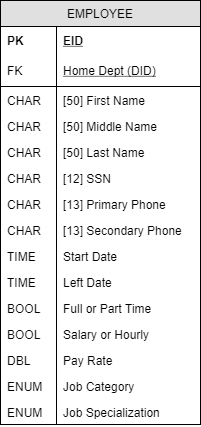
\includegraphics[scale=.6]{employee.png}
\end{figure}
\newpage
As you may have noticed, the addresses were not handled in the employee table. In the case that the employee may have multiple addresses, this system allows you to store only as much information as needed for each employee. The address records store the associated employee's EID along with the standard address information.
\begin{figure}[H]
	\centering
	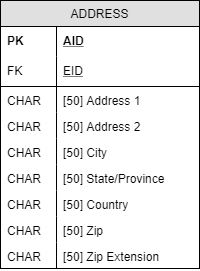
\includegraphics[scale=.6]{address.png}
\end{figure}

If an employee has relevant certifications, they can be linked to the employee by their EID within the certificate table.
\begin{figure}[H]
	\centering
	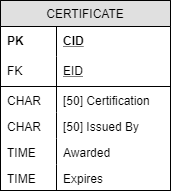
\includegraphics[scale=.6]{certificate.png}
\end{figure}

As requested, each department will have the ability to denote their staffing requirements by including a minimum and maximum number of employees required. The department charge nurse will also be linked to the department using their EID. The table will also record the number of beds in order to keep track of the ratio of staff to patients for that particular department utilizing a view within the database.
\begin{figure}[H]
	\centering
	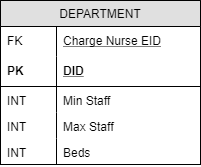
\includegraphics[scale=.6]{department.png}
\end{figure}

\newpage
With all of the necessary background tables out of the way, the following tables will concern all of the actual scheduling matter, starting with the table of weeks. This table simply lists the week's start and end dates in order to organize the shifts for that week.
\begin{figure}[H]
	\centering
	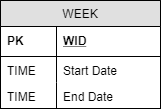
\includegraphics[scale=.6]{week.png}
\end{figure}

The shift table will become the most important table for creating views of the week's assignments. Each employee will be assigned multiple shifts per week, one for each shift they are scheduled to work. The shift requires the EID for the employee, the DID for the department and the WID of the week to show when, where and which employee will be working that shift. The day of the week will be selected through enumeration, as well as which shift out of the specified shifts they will be working for that day.

The status field will be used to denote one of the following: Called-in, Called-off, Requested-off, Requested-shift, none. In the case of schedule request conflicts, seniority will be used to determine which employee gets the shift. The pay increase is a decimal number (default of 1.00) indicating any shift differential the employee may receive from working a special shift (getting called in, nights or weekends) and will be applied to their pay rate when calculating the hours worked throughout the week.
\begin{figure}[H]
	\centering
	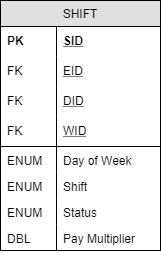
\includegraphics[scale=.6]{shift.png}
\end{figure}

Finally, the break table will be associated with the shift the employee is currently working. When employees clock out and clock in, the times will be recorded and the total time will be calculated and shown when a shift report is generated.
\begin{figure}[H]
	\centering
	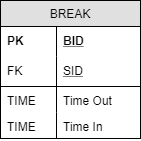
\includegraphics[scale=.6]{break.png}
\end{figure}

\newpage

When adding shifts for each employee, a two week period is examined and checked to see if they already have 12 shifts scheduled. If so, they will not be allowed to have any more shifts scheduled for that period. A similar procedure follows for adding shifts to a particular week; that week is checked to see if two 8-hour shifts or one 12-hour shift is already assigned to that employee for the day in question.

Summaries will be generated upon request to the database for displaying a full week's schedule. Views will also be implemented to show which full time employees that have less than 5 shifts for a given week, which departments are under- or over-staffed and to generate a payroll for all employees based on their pay rates, multiplied by their shift pay increase.

\bigskip{}\decorativeline\bigskip{}

Sincerely,\\

\quad Kyle Salitrik

\newpage
\begin{figure}[H]
	\centering
	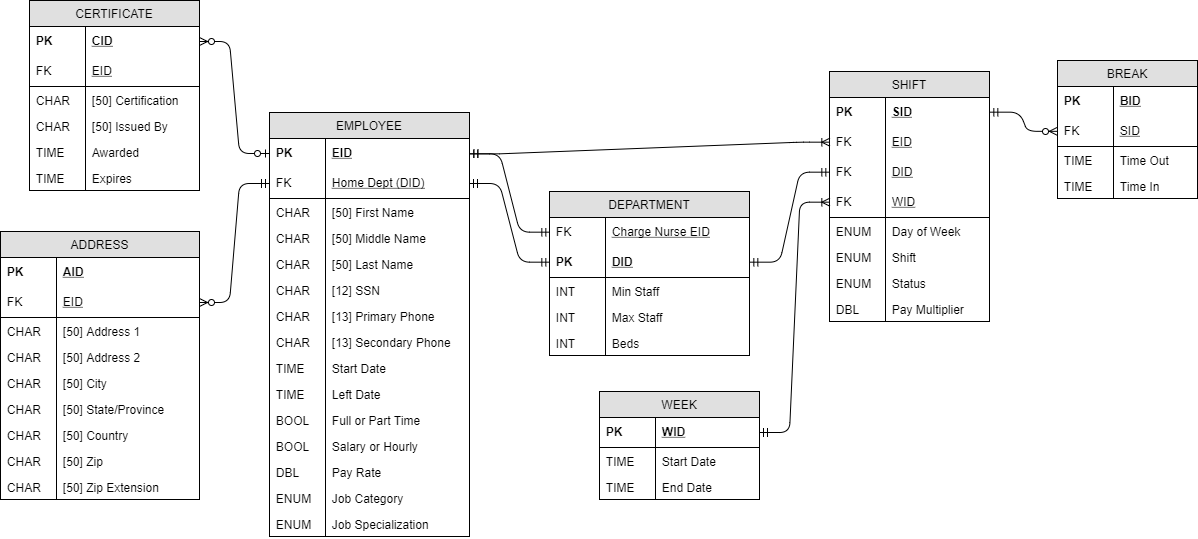
\includegraphics[angle=90, height=\textheight]{er_diag.png}
\end{figure}

\end{document}